

\chapter{Reconhecimento Facial}

	Algo explicando o que terá nesse capítulo.

\section{Biometria}

As abordagens de identificação pessoal que utilizam ``alguma coisa que você sabe'', como Número de Indetificação Pessoal (PIN - ``Personal Identification Number''), ou ``alguma coisa que você tenha'', como um cartão de identificação, não são confiáveis o suficiente para satisfazer os requisitos de segurança de um sistema de transações eletrônicas porque não têm a capacidade de diferenciar um usuário legítimo de um impostor que adiquiriu de forma ilegal o privilégio de acesso \cite{hong}. Esta fragilidade pode ser evitada se utilzarmos o nosso corpo como chave do sistema. Alguns traços fisícos ou comportamentais são muito mais complicados de serem forjados que uma cadeia de caracteres \cite{drovetto}.

Biometria é uma tecnologia utilizada para identificação de um indivíduo baseado em suas características físicas ou comportamentais, baseia-se em ``alguma coisa que você é ou faz'' para realizar a identificação e, por isso, tem a capacidade de diferenciar entre um indivíduo legítimo de um impostor \cite{hong}. As características físicas estão relacionadas a composição do corpo humano e seu formato e as comportamentais estão relacionadas ao comportamento das pessoas \cite{drovetto}. A figura \ref{caracteristicasBiometricas}contém alguns exemplos desses dois tipos diferentes de características biométricas.

	\begin{figure}[hbt]
		\begin{center}
			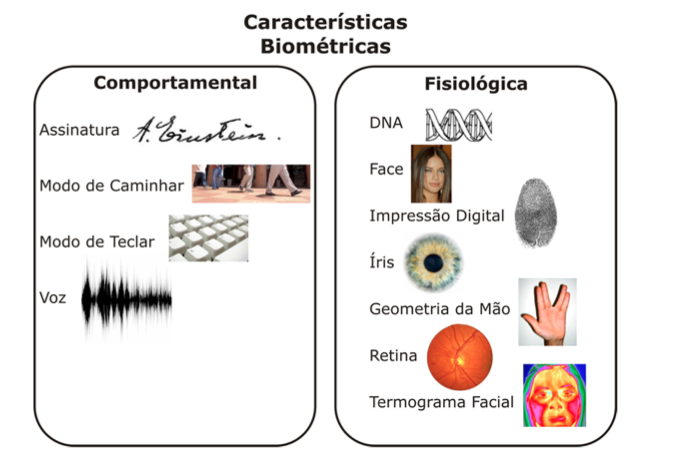
\includegraphics[height=11cm,width=17cm]{figuras/2.FundamentacaoTeorica/caracteristicasBiometricas.png}
		\end{center}
		\caption{Exemplos de algumas características biométricas \cite{drovetto}.}
		\label{caracteristicasBiometricas}
	\end{figure}

Teoricamente, qualquer característica física/comportamental pode ser utilizada para identificação caso siga alguns dos seguintes requisitos \cite{milene}: 

	\begin{enumerate}
		\item \textbf{universidade}: qualquer pessoa pode ser avaliada sobre essa característica;
		\item \textbf{singularidade}: dada duas pessoas distinas, elas não podem ter a mesma característica;
		\item \textbf{permanência}: a característica não pode mudar de acordo com o tempo;
		\item \textbf{exigibilidade}: significa que a característica pode ser mensurada quantitativamente;
	\end{enumerate}

Porém, na prática também são considerados outros requisitos \cite{milene}:

	\begin{enumerate}
		\item \textbf{desempenho}: o processo de identificação deve apresentar um resultado aceitável;
		\item \textbf{aceitação}: indica em que ponto as pessoas estão dispostas a aceitar o sistema biométrico;
		\item \textbf{evasão}: refere a facilidade de ser adulterado;
	\end{enumerate}

São várias as vatangens que os sistemas biométricos têm em relação aos sistemas convencionais. Listamos as vatagens vistas como principais \cite{drovetto}:
	
	\begin{itemize}
		\item características biométricas não podem ser perdidas ou esquecidas;
		\item características biométricas são difíceis de serem copiadas, compartilhadas e distribuídas;
		\item os sistemas biométricos necessitam que a pessoas esteja presente no local da autenticação;
	\end{itemize}

Novas técnicas de reconhecimento por meio de faces, íris, retina e voz, entre outras, têm sido abordadas para aplicações em sistemas de reconhecimento automático \cite{bolle,saocarlos}. O reconhecimento facial é apenas uma das nove características biométricas utilizadas atualmente \cite{milene}. Nas tabelas \ref{tabelaRequisitosTeoricos} e \ref{tabelaRequisitosPraticos} são mostradadas as noves características e seus respectivos comportamentos baseados nos requisitos mencionados acima.
		
	\begin{table}[htb]
		\begin{center}
			\caption{Requisitos teóricos para algoritmos de reconhecimento facial \cite{milene}.}
			\begin{tabular}{|c|c|c|c|c|}
				\hline \bf Biometria & \bf Universidade & \bf Singularidade & \bf Permanência & \bf Exigibilidade \\
				\hline \hline \bf Face & Alta & Baixa & Média & Alta \\
				\hline \bf  Digital & Média & Alta & Alta & Média \\
				\hline \bf Geometria da Mão & Média & Média & Média & Alta \\
				\hline \bf ``Hand Vein'' & Média & Média & Média & Média \\
				\hline \bf Iris & Alta & Alta & Alta & Média \\
				\hline \bf ``Retina Scan'' & Alta & Alta & Média & Baixa \\
				\hline \bf Assinatura & Baixa & Baixa & Baixa & Alta\\
				\hline \bf Voz & Média & Baixa & Baixa & Média \\
				\hline \bf Termograma & Alta & Alta & Baixa & Alta \\
				\hline
			\end{tabular}
		\end{center}
		\label{tabelaRequisitosTeoricos}
	\end{table}

	\begin{table}[htb]
		\begin{center}
			\caption{Requisitos práticos para algoritmos de reconhecimento facial \cite{milene}.}
			\begin{tabular}{|c|c|c|c|}
				\hline \bf Biometria & \bf Desempenho & \bf Aceitação & \bf Evasão \\
				\hline \hline \bf Face & Baixa & Alta & Baixa\\
				\hline \bf Digital & Alta & Média &  Alta\\
				\hline \bf Geometria da Mão & Média & Média & Média\\
				\hline \bf ``Hand Vein'' & Média & Média & Alta\\
				\hline \bf Iris  & Média & Média & Alta\\
				\hline \bf ``Retina Scan'' & Alta & Baixa & Alta\\
				\hline \bf Assinatura & Baixa & Alta & Baixa \\
				\hline \bf Voz & Baixa & Alta & Baixa \\
				\hline \bf Termograma & Média & Alta & Alta \\
				\hline
			\end{tabular}
		\end{center}
		\label{tabelaRequisitosPraticos}
	\end{table}

Um sistema biométrico responde a dois eventos: um usuário é ou não quem afirma ser. Como resposta a esses eventos, o sistema pode classificar o usuário como um cliente ou um impostor. Nessa tomada de decisão pode ocorrer dois tipos de erros: uma falsa aceitação, ao aceitar um impostor, (\textit{False Acceptance} - FA) ou uma falsa rejeição (\textit{False Rejection} - FR), ao rejeitar um cliente. Baseado nesses erros, duas taxas são utilizadas para avaliar sistemas biométricos: taxa de falsa aceitação (\textit{False Acceptance Rate} - FAR) e taxa de falsa rejeição (\textit{False Rejection Rate} - FRR) \cite{drovetto}.

A FAR é a probabilidade de um sistema biométrico aceitar um impostor como cliente. Ela é calculada pela equação (2.1) em que $\displaystyle Nfa$ é o número de falsas aceitações e $\displaystyle Ni$ é o número de impostores que tentaram acessar o sistema. A variação da taxa é representada pelo intervalo fechado $\displaystyle [0,1]$, onde o valor $\displaystyle 1$ significa que todos os impostores foram falsamente aceitos e o valor $\displaystyle 0$ significa que todos impostores foram identificados como tao. Logo quando menor o FAR mais seguro o sistema é \cite{drovetto}.

	\begin{equation}
		FAR = \frac{Nfa}{Ni} \cite{drovetto}
	\end{equation} 

A FRR é a probabilidade de um sistema biométrico rejeitar um cliente e classifica-lo como impostor. Ela é calculada pela equação (2.2) em que $\displaystyle Nfr$ é o número de falsas rejeições e $\displaystyle Nc$ é o número de clientes que tentaram acessar o sistema. A variação da taxa é representada pelo intervalo fechado $\displaystyle [0,1]$, onde o valor $\displaystyle 1$ significa que todos os clientes foram falsamente rejeitados e o valor $\displaystyle 0$ significa que todo os cliente foram aceitos corretamente. Em sistemas cuja performance tem maior grau de prioridade que a segurança, deve-se reduzir a FRR para minimizar a ocorrência de falsas rejeições \cite{drovetto}.

	\begin{equation}
		FRR = \frac{Nfr}{Nc} \cite{drovetto}
	\end{equation} 

A partir dessas taxas de erro, pode-se obter outras medidas como a \textit{Equal Error Rate} (ERR). Esta corresponde a taxa de erro na qual a tanto a FAR quanto a FRR possuem o mesmo valor. Como diferentes sistemas têm comportamentos diferentes, a ERR normalmente é utilizada para uma comparação mais rigorosa entre o sistemas. Quanto menor for a ERR, mas presciso é considerado o sistema \cite{drovetto}.

\section{Reconhecimento Facial}

Um dos motivos que icentivou os diversos estudos sobre reconhecimento facial são as vantagens que o mesmo possui em relação a impressão digital e a íris.  No reconhecimento por impressão digital, a desvantagem consiste no fato que nem todas as pessoas possuem uma impressão digital com ``qualidade'' suficiente para ser reconhecida por um sistema. Já o reconhecimento por íris apresenta uma alta confiabilidade e larga variação, sendo estável pela vida toda. Porém, a desvantagem está relacionada ao modo de captura da íris que necessita de uma alinhamento entre a câmera e os olhos da pessoa \cite{saocarlos}.

No anos 70, os estudos do reconhecimento facial eram baseados sobre atributos faciais mensuráveis como olhos, nariz, sobrancelhas, bocas, entre outros. Porém, os recursos computacionais eram escassos e os algoritmos de extração de características eram ineficiêntes. Então, as pesquisas na área ressurgiram nos anos 90, inovando os métodos existentes \cite{hong, saocarlos}.







